%%%%%%%%%%%%%%%%%%%%%%%%%%%%%%%%%%%%%%%%%%%%%%%%%%%%%%%%%%%%%%%%%%%%%%%%%%%%%%%%%%%%%%%%%%

%%%%%%%%%%%%%%%%%%%%%%%%%%%%%%%%%%% Author:Yao Zhang  %%%%%%%%%%%%%%%%%%%%%%%%%%%%%%%%%%%%
%%%%%%%%%%%%%%%%%%%%%%%%%%%%% Email: jaafar_zhang@163.com  %%%%%%%%%%%%%%%%%%%%%%%%%%%%%%%

%%%%%%%%%%%%%%%%%%%%%%%%%%%%%%%%%%%%%%%%%%%%%%%%%%%%%%%%%%%%%%%%%%%%%%%%%%%%%%%%%%%%%%%%%%

\documentclass[aspectratio=2516]{beamer}
\mode<presentation> {
\usetheme{Madrid}
%\setbeamertemplate{footline} % To remove the footer line in all slides uncomment this line
}

\usepackage{graphicx} 
\graphicspath{ {img/} }
\usepackage[caption=false, font=footnotesize]{subfig}
\setbeamertemplate{caption}[numbered]
\newtheorem{remark}{Remark}
\newtheorem{coro}{Corollary}
\newtheorem{thm}{Theorem}
\newtheorem{eg}{Example}
\newtheorem{proposition}{Proposition}
\newtheorem{lma}{Lemma}
\usepackage{algorithm}
\usepackage{algorithmic}
\renewcommand{\algorithmicrequire}{\textbf{Input:}}  
\renewcommand{\algorithmicensure}{\textbf{Output:}} 
\setbeamertemplate{theorems}[numbered]
\usepackage{bbding}
%\usepackage{ctex}
\renewcommand{\figurename}{Figure}
\renewcommand{\tablename}{Table}

%----------------------------------------------------------------------
\title[Follow Your Heart]{ When You Follow Your Heart} % The short title appears at the bottom of every slide, the full title is only on the title page
\vspace{0.5cm}
\subtitle{ You Cease Having Regrets}
\vspace{2.5cm}


\author{Yao Zhang} % 

\institute[UCAS \& NAOC] 
{	
%    Advisor: Dr. Long Xu \\
%    
%    \vspace{0.5cm}
    
    University of Chinese Academy of Sciences \\
     
	\vspace{0.2cm}
	
	 National Astronomical Observatories, Chinese Academy of Sciences \\
	 
	% \vspace{0.2cm}
	 
	%  {\color{blue} \tiny Joint work with Dr. M. Li (SZU), Dr. M. Xiao (SIUC),  Dr. L. Xu  (NAOC) and  Y. Yang (SZU)} \\
	 
	 \vspace{0.5cm}
	
     {\color{blue} \url{https://zhims.github.io}}
}

\date{\today}


\logo{
\includegraphics[height=0.6cm]{yao.jpg}}

%----------------------------------------------------------------------
\begin{document}
	\begin{frame}
	\titlepage 
	\end{frame}
%-----------------------------------------------------------------------
\begin{frame}
\frametitle{Overview} 
\begin{small}
	\tableofcontents
\end{small} 
\end{frame}

%----------------------------- section 1 -------------------------------------------
\section{Our Academic Family}
%-----------------------------------------------------------------------------------

\begin{frame}
\frametitle{ Section \uppercase\expandafter{\romannumeral1}}


\begin{center}
	\Large Our Academic Family
\end{center}

\end{frame}
%------------------------------------------------------------------------------------

\begin{frame}
\frametitle{Our Academic Family}


\begin{figure}
	\centering
	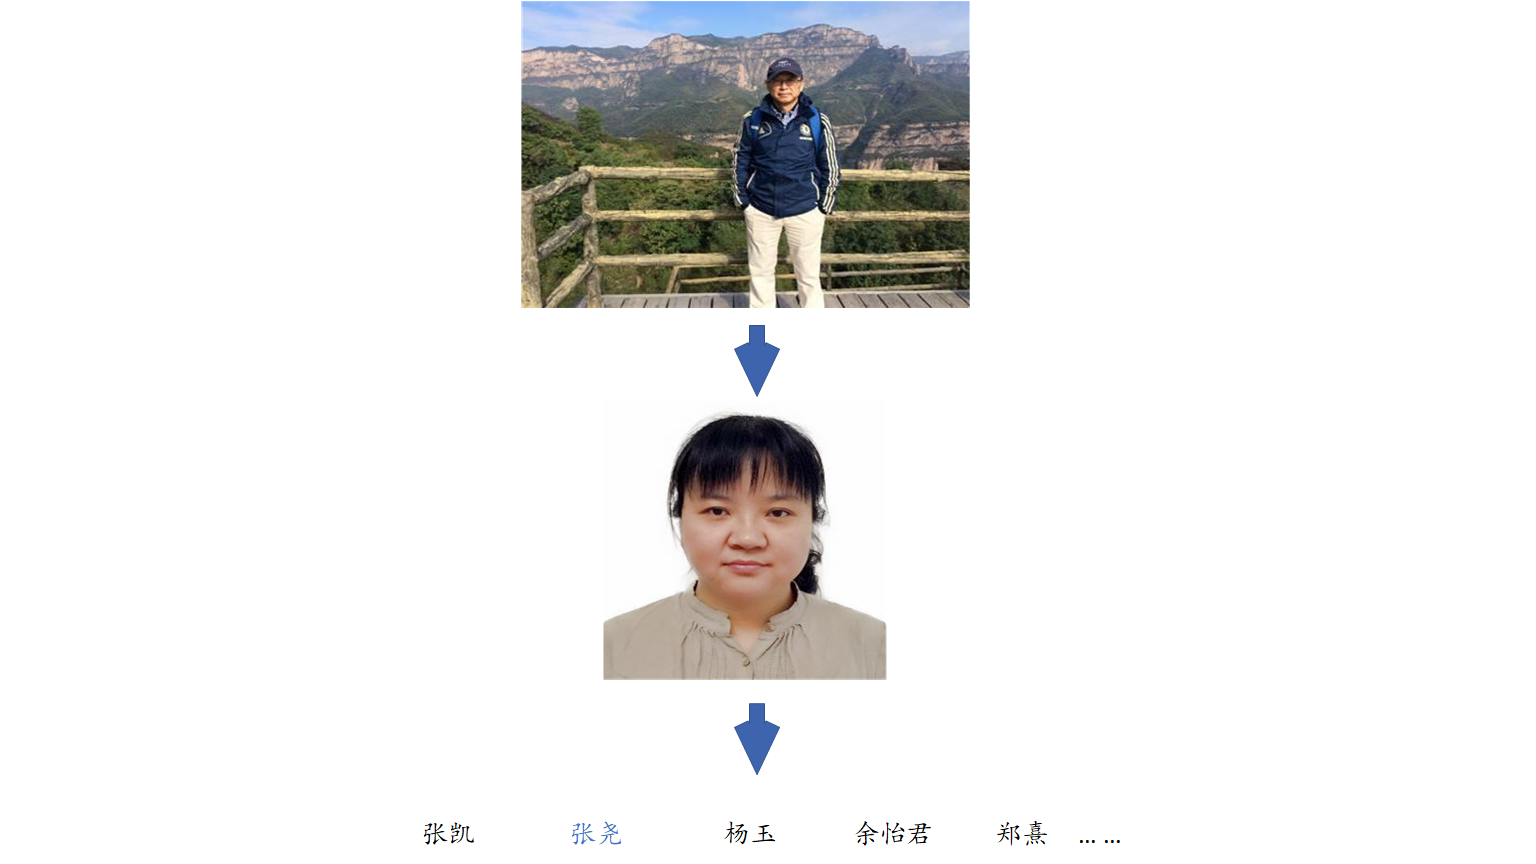
\includegraphics[width=0.9\linewidth,height=0.5\linewidth]{yao_zhang.png}
	\caption{Our Academic Family}
	\label{fig1} 
\end{figure}

\end{frame}



%-----------------------------------------------------------------------------------

%-----------------------------------------------------------------------------------

%----------------------------- section 2 -------------------------------------------
\section{How to Read a Scientific Paper}
%-----------------------------------------------------------------------------------

\begin{frame}
\frametitle{ Section \uppercase\expandafter{\romannumeral2}}


\begin{center}
	\Large How to Read a Scientific Paper?
\end{center}

\end{frame}

%-----------------------------------------------------------------------------------

\begin{frame}
	\frametitle{How to Read a Scientific Paper?}
	
	In my personal opinion:
	
	\vspace{0.5cm}
	
	\begin{enumerate}
		\item  What are the basic assumptions of the model mentioned in the paper?
		
		\vspace{0.5cm}
		
		\item  How to check scientific assumptions of the model mentioned in the paper?
		
		\vspace{0.5cm}
		
		\item  How to generalize from  finite to infinity?
		
		\vspace{0.5cm}
		
		\item  Computation and Proof  again and again. 
		
		\vspace{0.5cm}
		
		\item  $ \cdots $
		
	\end{enumerate}
	
	\vspace{0.25cm}
	
	{\tiny There is a recommended paper: \ {\color{blue} \url{https://web.stanford.edu/class/cs244/papers/HowtoReadPaper.pdf}}}.
\end{frame}
%-----------------------------------------------------------------------------------

%----------------------------- section 3 -------------------------------------------
\section{How to Build a Fine Life}
%-----------------------------------------------------------------------------------

\begin{frame}
	\frametitle{ Section \uppercase\expandafter{\romannumeral3}}
	
	
	\begin{center}
		\Large How to Build a Fine Life?
	\end{center}
	
\end{frame}

%-----------------------------------------------------------------------------------
\begin{frame}
	\frametitle{How to Build a Fine Life}
	\begin{enumerate}
		
		\item Stop keeping score.
		
		\vspace{0.5cm}
		
		\item Find the place you love.
		
		\vspace{0.5cm}
		
		\item Don’t isolate yourself.
		
		\vspace{0.5cm}
		
		\item Sedentary pandemic life is bad for our happiness.
		
		\vspace{0.5cm}
		
		\item $ \cdots $
		
	\end{enumerate}

\vspace{0.25cm}

{\tiny There is a recommended website: \ {\color{blue} \url{https://www.theatlantic.com/projects/how-build-life/}}}.
\end{frame}

%-----------------------------------------------------------------------------------

%----------------------------- section 4 -------------------------------------------
\section{How to Take Notes}
%-----------------------------------------------------------------------------------

\begin{frame}
	\frametitle{ Section \uppercase\expandafter{\romannumeral4}}
	
	\begin{center}
		\Large How to Take Notes?
	\end{center}
	
\end{frame}

%-----------------------------------------------------------------------------------
\begin{frame}
	\frametitle{How to Take Notes?}
	\begin{enumerate}
		
		\item \LaTeX: {\color{blue} \url{https://tug.org/texlive/}}
		
		\vspace{0.75cm}
		
		\item TeXstudio: {\color{blue} \url{https://www.texstudio.org/}}
		
		\vspace{0.75cm}
		
		\item Overleaf: {\color{blue} \url{https://www.overleaf.com/}}
		
		\vspace{0.75cm}
		
		\item MathType
		
	\end{enumerate}
\end{frame}

%-----------------------------------------------------------------------------------

%----------------------------- section 5 -------------------------------------------
\section{How to Code}
%-----------------------------------------------------------------------------------

\begin{frame}
	\frametitle{ Section \uppercase\expandafter{\romannumeral5}}
	
	\begin{center}
		\Large How to Code?
	\end{center}
	
\end{frame}

%-----------------------------------------------------------------------------------
\begin{frame}
	\frametitle{How to Take code?}
	\begin{enumerate}
		
		\item Matlab
		
		\vspace{0.75cm}
		
		\item Python 
		
		\vspace{0.25cm}
		
		\begin{enumerate}
			\item PyTorch
			
			\vspace{0.25cm}
			
			\item  Pillow
			
			\vspace{0.25cm}
			
			\item  Anaconda 
		\end{enumerate}
		
		\vspace{0.75cm}
		
		\item Debug and Code
		
	\end{enumerate}
\end{frame}

%-----------------------------------------------------------------------------------

%----------------------------- section 6 -------------------------------------------
\section{Are Books Still Important?}
%-----------------------------------------------------------------------------------

\begin{frame}
	\frametitle{ Section \uppercase\expandafter{\romannumeral6}}
	
	\begin{center}
		\Large Are Books Still Important?
	\end{center}
	
\end{frame}

%-----------------------------------------------------------------------------------
\begin{frame}
	\frametitle{Are Books Still Important?}
	
	\begin{center}
		{\color{blue} \Large Yes!}
	\end{center}

{\small  There are some recommended books:}

\vspace{0.25cm}

\begin{enumerate}
	\item {\small Deep Learning Architectures}:
	
	{\tiny \color{blue}\url{https://www.springer.com/gp/book/9783030367206}}.
	
	\vspace{0.25cm}
	
	\item {\small Understanding Machine Learning: From Theory to Algorithms}:
	
	{\tiny \color{blue} \url{https://www.cs.huji.ac.il/~shais/UnderstandingMachineLearning/}}.
	
	\vspace{0.25cm}
	
	\item {\small Matrix Computation (in Chinese)}:
	
	{\tiny \color{blue} https://item.jd.com/13016640.html}.
	
	\vspace{0.25cm}
	
	\item {\small High-Dimensional Data Analysis with Low-Dimensional Models: Principles, Computation, and Applications}.
	
	{\tiny \color{blue} \url{https://book-wright-ma.github.io/Book-WM-20201206.pdf}}.
	
	\item $ \cdots  $
\end{enumerate}

\end{frame}


%-------------------------------------------------------------------------------------------
\begin{frame}
\frametitle{The End}
\begin{center}
	{\Huge Thank you!}
	
	\vspace{1cm}
	
	{\Huge Any comments or questions?}
	
	\vspace{2.25cm}	
	
  {\tiny Welcome to visit my personal homepage: \ {\color{blue} \url{https://zhims.github.io/}}}
\end{center}
\end{frame}
%----------------------------------------------------------------------------------------
%----------------------------------------------------------------------------------------

\end{document} 